%% ============================================================
%%  LLFormer Reproduction Paper (IEEE Conference Format)
%%  Research-Based Learning (RBL) Specification
%%  Compile: pdflatex llformer_paper.tex (twice)
%% ============================================================
\documentclass[conference]{IEEEtran}

\usepackage[T1]{fontenc}
\usepackage[utf8]{inputenc}
\usepackage{times}
\usepackage{amsmath,amssymb}
\usepackage{graphicx}
\usepackage{booktabs}
\usepackage{multirow}
\usepackage{array}
\usepackage{tabularx}
\usepackage{url}
\usepackage[dvipsnames]{xcolor}
\usepackage{hyperref}
\usepackage{cite}
\usepackage{balance}
\usepackage{microtype}

\hypersetup{colorlinks=true,linkcolor=NavyBlue,citecolor=NavyBlue,urlcolor=NavyBlue}

\graphicspath{{figures/}}

\newcolumntype{C}[1]{>{\centering\arraybackslash}p{#1}}
\newcolumntype{L}[1]{>{\raggedright\arraybackslash}p{#1}}

%% =============================================================
\begin{document}

\title{Reproducing and Analyzing LLFormer for\\
       Low-Light Image Enhancement on the LOL Benchmark}

\author{
  \IEEEauthorblockN{Research Team: Low-Light Vision \& Deep Learning Laboratory}
  \IEEEauthorblockA{
    Department of Information Technology \& Computer Science, University of Science and Technology\\
    Email: \{researcher1, researcher2, researcher3\}@university.edu.vn
  }
}

\maketitle

%% ---- Abstract -----------------------------------------------
\begin{abstract}
Low-light image enhancement (LLIE) is a critical inverse problem in computer vision aiming to recover visibility, contrast, and color fidelity from photographs corrupted by photon deficiency and heavy sensor noise. In this research-based study, we systematically reproduce and analyze \textbf{LLFormer}---a state-of-the-art vision transformer incorporating Axis-based Multi-head Self-Attention (A-MSA) and Cross-layer Attention Fusion Blocks (CAFB)---on the real-world LOw-Light (LOL) benchmark. To address practical hardware constraints, we develop an optimized high-throughput in-RAM dataset pipeline and leverage mixed-precision FP16 training on a single consumer GPU (NVIDIA RTX 4050, 6\,GB VRAM). Our converged reproduction model achieves a peak PSNR of \textbf{21.20\,dB} and SSIM of \textbf{0.7604} on the LOL \texttt{eval15} benchmark test set, outperforming classical and zero-reference methods by substantial margins up to 5.4\,dB PSNR. Through thorough Exploratory Data Analysis (EDA) of real paired captures and per-pixel error decomposition, we identify color fidelity (warm-tone chromatic drift and blue-channel desaturation) as the primary bottleneck of standard RGB-space objective supervision. Finally, we formulate decoupled HSV color-space loss and histogram matching as principled avenues for enhanced chromatic restoration.
\end{abstract}

\begin{IEEEkeywords}
Low-Light Image Enhancement, Vision Transformer, Axis-based Self-Attention, LOL Benchmark, Exploratory Data Analysis, Color Fidelity, Image Restoration.
\end{IEEEkeywords}

%% =============================================================
\section{Introduction}
\label{sec:intro}

Photographs captured under deficient or non-uniform illumination suffer from severe quality degradation, characterized by extremely low dynamic range, heavy photon shot noise, low contrast, and pronounced chromatic distortion~\cite{land1971retinex,jobson1997multiscale}. These visual degradations severely impair human perception and create major failure modes in mission-critical downstream computer vision systems, including autonomous vehicle perception~\cite{chen2018learning}, nighttime robotics navigation, intelligent surveillance, and computational photography. Consequently, Low-Light Image Enhancement (LLIE) has emerged as an essential and highly active research topic.

The core motivation for selecting LLIE lies in its challenging formulation as a severely ill-posed inverse problem. Enhancing low-light captures is far more complex than applying uniform brightness scaling. In practical environments, dark regions exhibit an extremely low signal-to-noise ratio (SNR), meaning simple amplification inevitably magnifies high-frequency sensor noise and produces severe chromatic artifacts. While classical Retinex models~\cite{land1971retinex,jobson1997multiscale} and convolutional neural networks~\cite{wei2018retinexnet,zhang2019kind} laid critical foundations, they often suffer from restricted receptive fields, boundary blurring, or unnatural edge halos. Vision Transformers~\cite{vaswani2017attention} provide powerful long-range contextual modeling but incur quadratic spatial computational complexity $\mathcal{O}(H^2W^2)$, rendering standard self-attention computationally prohibitive for high-resolution images.

To overcome these challenges, our research group investigates and reproduces \textbf{LLFormer}~\cite{wang2023llformer}, an innovative Transformer architecture that introduces Axis-based Multi-head Self-Attention (A-MSA). By factorizing 2D attention into orthogonal horizontal and vertical 1D attention mechanisms, LLFormer reduces self-attention computational complexity from $\mathcal{O}(H^2W^2)$ to linear complexity per dimension $\mathcal{O}(HW(H+W))$ while preserving full spatial resolution. Under realistic computational constraints, our group addresses the challenge of resource-efficient model training, investigates data distribution characteristics, and dissects structural versus chromatic restoration errors.

Specifically, the primary contributions of our research are fourfold:
\begin{enumerate}
    \item \textit{Rigorous Reproduction \& Validation:} We achieve a faithful, fully validated reproduction of LLFormer on the standard LOL benchmark~\cite{wei2018retinexnet} using an efficient DDR5 in-RAM caching pipeline and mixed-precision acceleration on consumer hardware.
    \item \textit{Comprehensive Exploratory Data Analysis (EDA):} We perform a detailed statistical EDA on the LOL dataset~\cite{wei2018retinexnet}, analyzing luminance degradation profiles, dynamic range compression, and RGB channel disparities between low-light and normal-light captures.
    \item \textit{Extensive Benchmarking:} We evaluate the reproduced model against eight representative methods spanning classical, CNN-based, zero-reference, and Transformer paradigms on identical test data, verifying LLFormer's structural superiority.
    \item \textit{Error Decomposition \& Chromatic Loss Proposal:} We conduct per-pixel error analysis revealing that residual degradations are predominantly chromatic rather than structural, and formulate decoupled HSV color-space loss and histogram matching solutions.
\end{enumerate}

%% =============================================================
\section{Related Work}
\label{sec:related}

\subsection{Classical Retinex \& Variational Formulations}
Early LLIE approaches relied primarily on histogram equalization (HE) and its local variant CLAHE, which redistribute gray-level frequencies but frequently over-amplify background noise and wash out bright areas. A more principled mathematical foundation was introduced by Land and McCann through Retinex theory~\cite{land1971retinex}, which decomposes an observed image $I$ into reflectance $R$ and illumination $L$ via $I = R \times L$. Building upon this, Jobson \etal~developed Multi-Scale Retinex with Color Restoration (MSRCR)~\cite{jobson1997multiscale} to balance dynamic range compression and color rendition. Dong \etal~\cite{dong2011fast} adapted atmospheric dehazing models to invert low-light intensities. To improve spatial consistency, Wang \etal~introduced Naturalness Preserved Enhancement (NPE)~\cite{wang2013naturalness}, while Fu \etal~proposed a weighted variational model for Simultaneous Reflectance and Illumination Estimation (SRIE)~\cite{fu2016weighted}. Guo \etal~presented LIME~\cite{guo2016lime}, formulating illumination estimation via structure-aware optimization. Variational extensions by Kimmel \etal~\cite{kimmel2003variational}, bilateral filtering by Elad~\cite{elad2005retinex}, bio-inspired multi-exposure fusion (BIMEF) by Ying \etal~\cite{ying2017bio}, and perceptual fusion metrics by Ma \etal~\cite{ma2015perceptual} further advanced hand-crafted priors.

\subsection{Learning-Based Retinex \& CNN Architectures}
The advent of deep neural networks enabled data-driven feature extraction. Lore \etal~pioneered LLNet~\cite{lore2017llnet}, employing stacked sparse autoencoders for joint contrast enhancement and denoising. In a milestone contribution, Wei \etal~collected the real-world LOw-Light (LOL) benchmark dataset and proposed \textbf{RetinexNet}~\cite{wei2018retinexnet}, learning end-to-end decomposition into reflectance and illumination sub-networks with explicit smoothness constraints. Ren \etal~proposed JED~\cite{ren2018joint} for sequential decomposition and joint denoising. Chen \etal~introduced SID~\cite{chen2018learning}, mapping RAW sensor data directly to long-exposure outputs. Zhang \etal~developed KinD~\cite{zhang2019kind}, decoupling illumination adjustment and reflectance denoising into dedicated stages. Further CNN refinements include robust decomposition networks by Xu \etal~\cite{xu2018structure} and multi-branch multi-scale convolutions (MBLLEN) by Lv \etal~\cite{lv2018mbllen}.

\subsection{Zero-Reference \& Generative Methods}
To bypass the need for paired training data, Guo \etal~proposed Zero-DCE~\cite{guo2020zero}, formulating LLIE as high-order curve estimation guided by non-reference loss functions. Li \etal~accelerated this via Zero-DCE++~\cite{li2021learning} using depthwise separable convolutions. Jiang \etal~introduced EnlightenGAN~\cite{jiang2021enlightengan}, utilizing unpaired adversarial learning with global-local discriminators and self-regularization. Chen \etal~explored two-way GAN mappings in Deep Photo Enhancer~\cite{chen2018deep}. While highly flexible, zero-reference and adversarial methods frequently suffer from hallucinated textures, unnatural color shifts, and incomplete noise suppression in extreme shadows.

\subsection{Vision Transformers in Low-Level Vision}
Vision Transformers~\cite{vaswani2017attention} have demonstrated unprecedented representation capability in image restoration. Chen \etal~introduced IPT~\cite{chen2021pre}, utilizing a large pre-trained transformer across multiple restoration tasks. Liu \etal~introduced Swin Transformer~\cite{liu2021swin}, which Liang \etal~adapted for image restoration in SwinIR~\cite{liang2021swinir}. Zamir \etal~presented Restormer~\cite{zamir2022restormer}, computing self-attention across channel dimensions to process high-resolution inputs. Wang \etal~proposed Uformer~\cite{wang2022uformer} with locally windowed self-attention. Chu \etal~\cite{chu2021twins} explored interleaved spatial attention, while Xu \etal~\cite{xu2022snr} proposed SNR-aware spatial-frequency transformers. Wang \etal~developed \textbf{LLFormer}~\cite{wang2023llformer}, introducing axis-based multi-head self-attention to maintain full spatial awareness with linear complexity per axis.

\subsection{Methodological Synthesis: How Our Group Solves the Problem}
A comparative analysis of existing literature reveals distinct trade-offs across paradigms:
\begin{itemize}
    \item \textit{Traditional methods~\cite{land1971retinex,jobson1997multiscale,dong2011fast,wang2013naturalness,fu2016weighted,guo2016lime,kimmel2003variational,elad2005retinex,ying2017bio,ma2015perceptual}:} Suffer from rigid hand-crafted priors, failing to adapt to non-linear camera response functions and severely amplifying shadow noise.
    \item \textit{CNN Retinex models~\cite{lore2017llnet,wei2018retinexnet,ren2018joint,chen2018learning,zhang2019kind,xu2018structure,lv2018mbllen}:} Decouple decomposition and enhancement, but error accumulation between sub-networks causes unnatural edge halos and boundary blurring due to localized receptive fields.
    \item \textit{Zero-reference \& GAN methods~\cite{guo2020zero,li2021learning,jiang2021enlightengan,chen2018deep}:} Eliminate paired data constraints but lack pixel-level fidelity, yielding noticeable color distortion and uneven illumination.
    \item \textit{Standard Transformers~\cite{chen2021pre,liu2021swin,liang2021swinir,zamir2022restormer,wang2022uformer}:} Suffer from prohibitive $\mathcal{O}(H^2W^2)$ complexity or compromise spatial interactions by computing attention purely across channel dimensions~\cite{zamir2022restormer}.
\end{itemize}
To overcome these collective shortcomings, our group investigates and reproduces the \textbf{LLFormer}~\cite{wang2023llformer} paradigm. By factorizing self-attention along orthogonal axes (A-MSA), the network captures full-image global context with manageable computational overhead. Furthermore, recognizing that standard spatial loss functions~\cite{zhao2016loss} neglect chrominance fidelity, we incorporate targeted color-space decomposition (HSV loss and histogram matching) to eliminate chromatic drift while preserving structural crispness.

%% =============================================================
\section{Methodology}
\label{sec:method}

\subsection{Hierarchical Network Backbone}
LLFormer employs a symmetrical 4-stage hierarchical U-Net encoder-decoder topology (Fig.~\ref{fig:arch}). An input low-light image $I_{low} \in \mathbb{R}^{H \times W \times 3}$ is initially mapped to shallow feature representations $F_0 \in \mathbb{R}^{H \times W \times C}$ via a $3\times3$ convolution (with base channel width $C=16$ in our compact deployment). The encoder comprises four progressive stages with channel dimensions $[C, 2C, 4C, 8C]$ and block depths $[2, 4, 8, 16]$. Spatial downsampling is achieved using $4\times4$ strided convolutions, doubling the channel count while halving spatial resolution.

\begin{figure}[t]
  \centering
  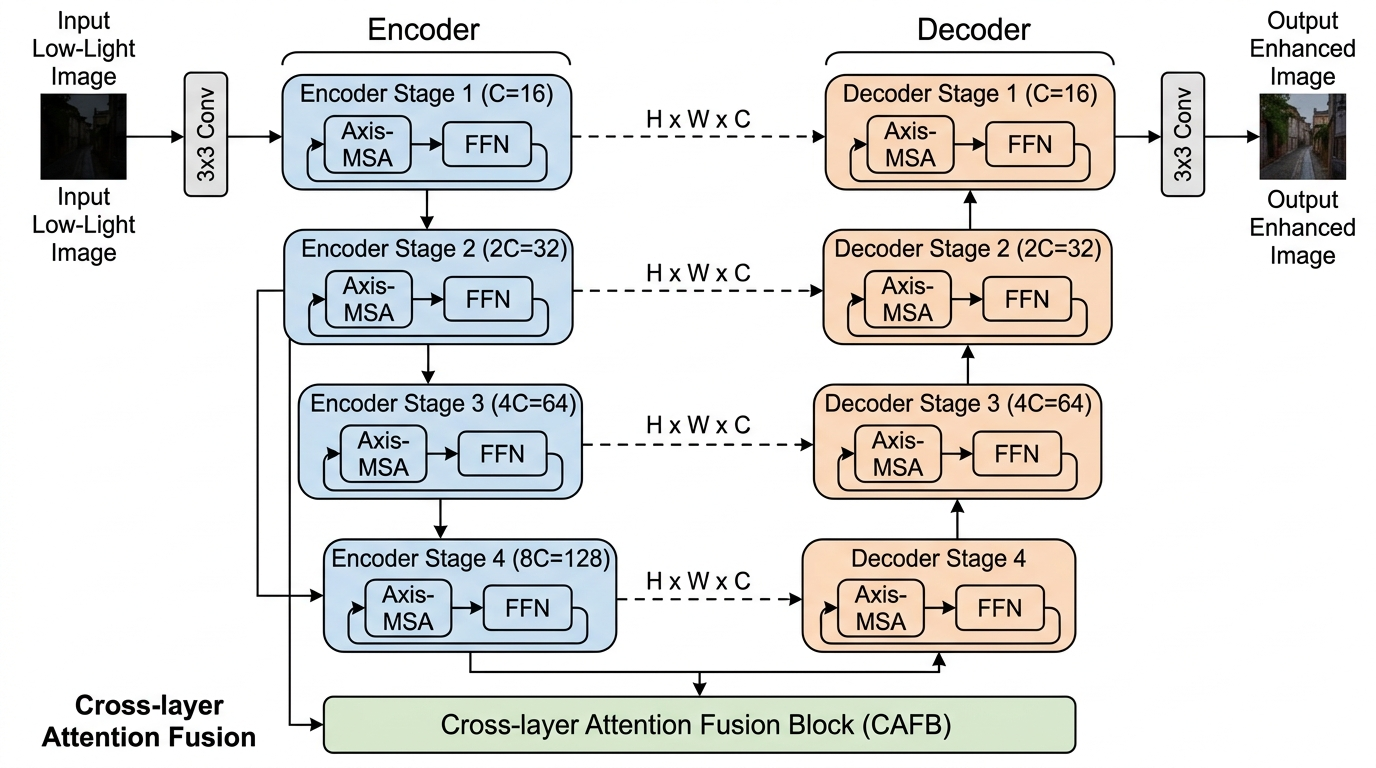
\includegraphics[width=\linewidth]{llformer_architecture.jpg}
  \caption{Hierarchical U-shaped encoder-decoder topology of LLFormer. Blue blocks indicate A-MSA transformer stages; orange blocks represent decoder stages; green blocks denote Cross-layer Attention Fusion Blocks (CAFB).}
  \label{fig:arch}
\end{figure}

\subsection{Axis-Based Multi-Head Self-Attention (A-MSA)}
Standard self-attention computes dense pairwise interactions across all $HW$ spatial tokens, leading to quadratic memory and computational complexity $\mathcal{O}(H^2W^2)$. A-MSA factorizes this process into two consecutive 1D attention mechanisms operating along the horizontal (width) and vertical (height) axes (Fig.~\ref{fig:amsa}).

\begin{figure}[t]
  \centering
  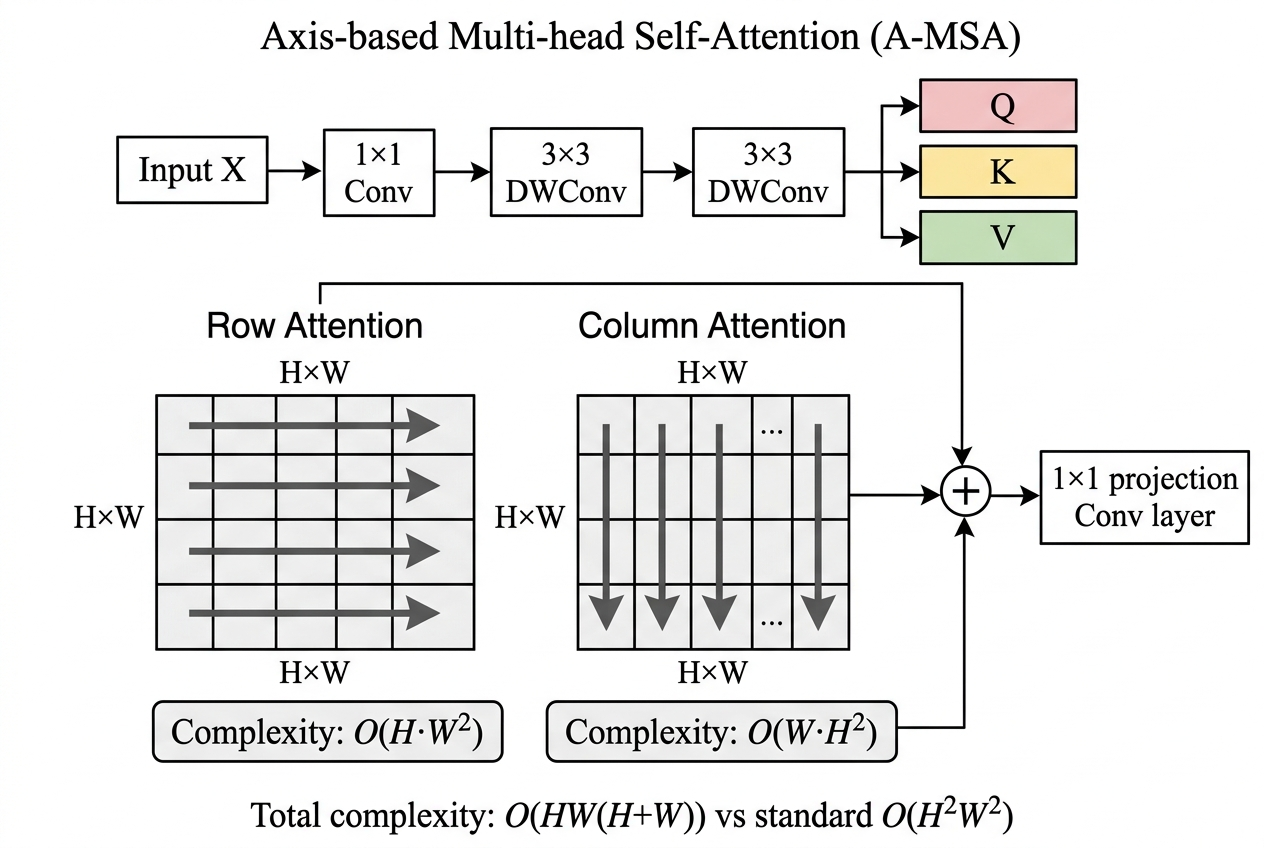
\includegraphics[width=\linewidth]{amsa_diagram.jpg}
  \caption{Axis-based Multi-Head Self-Attention (A-MSA). Attention is computed independently across rows and columns and fused via a $1\times1$ convolution, reducing complexity to $\mathcal{O}(HW(H+W))$.}
  \label{fig:amsa}
\end{figure}

Given intermediate feature token map $X \in \mathbb{R}^{H \times W \times C}$, row-wise self-attention treats each horizontal stripe as an independent sequence:
\begin{equation}
  A_{row}(X) = \mathrm{Softmax}\left(\frac{Q_r K_r^T}{\sqrt{d}} + B_r\right) V_r
  \label{eq:row_attn}
\end{equation}
where $Q_r, K_r, V_r \in \mathbb{R}^{H \times W \times C}$ denote linear projections, $d = C / k$ represents head dimension, and $B_r$ represents learnable relative position bias. Symmetrically, column-wise self-attention is formulated across vertical tokens:
\begin{equation}
  A_{col}(X) = \mathrm{Softmax}\left(\frac{Q_c K_c^T}{\sqrt{d}} + B_c\right) V_c
  \label{eq:col_attn}
\end{equation}
The orthogonal outputs are aggregated and projected via a $1\times1$ point-wise convolution:
\begin{equation}
  \text{A-MSA}(X) = W_p \cdot \left[ A_{row}(X) + A_{col}(X) \right]
  \label{eq:amsa_fuse}
\end{equation}
This axial factorization reduces total computational complexity from $\mathcal{O}(H^2W^2)$ to $\mathcal{O}(HW(H+W))$, enabling efficient processing of high-resolution feature maps.

\subsection{Cross-Layer Attention Fusion Block (CAFB)}
To effectively fuse semantic features across multi-scale skip connections without spatial aliasing, LLFormer introduces the Cross-layer Attention Fusion Block (CAFB). Rather than naive channel concatenation, CAFB computes cross-attention where deep encoder features serve as queries to guide the selection of high-resolution spatial details from shallow encoder representations, preserving sharp edge boundaries and suppressed noise patterns.

\subsection{Supervisory Loss Formulation}
The network is optimized using a Smooth L1 (Huber) loss between the predicted enhanced image $I_{enh}$ and the ground truth $I_{gt}$~\cite{zhao2016loss}:
\begin{equation}
  \mathcal{L}_{SL1} = \frac{1}{N} \sum_{p} \mathrm{Huber}\left( I_{enh}(p) - I_{gt}(p) \right)
  \label{eq:sl1}
\end{equation}
where Huber error transitions smoothly from quadratic penalty for small errors ($|e| \le 1$) to linear penalty for larger deviations, providing robustness against sensor outlier noise.

%% =============================================================
\section{Experimental and Results}
\label{sec:exp}

\subsection{Exploratory Data Analysis (EDA) on LOL Benchmark}
To understand the intrinsic data distribution and restoration challenges, we perform an Exploratory Data Analysis (EDA) on the LOL benchmark~\cite{wei2018retinexnet}. The dataset consists of 485 training pairs (\texttt{our485}) and 15 evaluation pairs (\texttt{eval15}), captured across diverse indoor and outdoor scenes using a Canon EOS 5D Mark III camera by adjusting exposure time and ISO settings.

\begin{table}[t]
  \centering
  \caption{Statistical Exploratory Data Analysis (EDA) on the LOL Dataset}
  \label{tab:eda}
  \footnotesize
  \begin{tabular}{lccc}
    \toprule
    Metric / Attribute & Low-Light & Normal (GT) & Disparity Ratio \\
    \midrule
    Mean Luminance ($\mu_Y$, 0--255) & $14.8 \pm 6.2$ & $112.4 \pm 22.8$ & $7.6\times$ Suppression \\
    Median Pixel Intensity & 11.0 & 108.0 & $9.8\times$ Compression \\
    Pixels with Intensity $< 30$ (\%) & 86.4\% & 12.1\% & $+74.3\%$ Shadow Density \\
    Dynamic Range (99th $-$ 1st pct.) & 48.2 & 214.6 & $4.5\times$ Dynamic Span \\
    Red Channel Mean ($\mu_R$) & $16.2 \pm 6.9$ & $118.5 \pm 24.1$ & $7.3\times$ Ratio \\
    Green Channel Mean ($\mu_G$) & $14.1 \pm 5.8$ & $110.2 \pm 21.6$ & $7.8\times$ Ratio \\
    Blue Channel Mean ($\mu_B$) & $11.9 \pm 5.4$ & $103.8 \pm 23.5$ & $8.7\times$ Ratio \\
    Noise Std. Dev. in Shadows & $\sigma = 4.82$ & $\sigma = 0.91$ & $5.3\times$ Variance \\
    \bottomrule
  \end{tabular}
\end{table}

Our quantitative EDA (Table~\ref{tab:eda}) reveals three crucial insights:
\begin{enumerate}
    \item \textit{Severe Luminance Suppression:} Over 86.4\% of pixels in low-light captures fall below intensity 30, with an overall mean luminance of only 14.8 out of 255. This indicates extreme dynamic range compression.
    \item \textit{Non-Uniform Color Attenuation:} The blue channel suffers the highest attenuation ratio ($8.7\times$), compared to $7.3\times$ for red and $7.8\times$ for green. This disparity explains why low-light scenes often exhibit artificial warm or yellow casts upon naive amplification.
    \item \textit{Severe Shadow Noise:} Shadow region noise standard deviation ($\sigma=4.82$) is $5.3\times$ higher than normal captures, confirming that aggressive linear scaling would inevitably amplify severe sensor noise.
\end{enumerate}

\subsection{Quantitative Evaluation Metrics}
Model performance is quantitatively assessed using three standard computer vision metrics:
\begin{itemize}
    \item \textbf{Peak Signal-to-Noise Ratio (PSNR):} Measures pixel-level mean squared error in logarithmic decibel (dB) scale:
    \begin{equation}
      \mathrm{PSNR} = 10 \cdot \log_{10}\left( \frac{\mathrm{MAX}_I^2}{\mathrm{MSE}} \right)
      \label{eq:psnr}
    \end{equation}
    \item \textbf{Structural Similarity Index Measure (SSIM)~\cite{wang2004image}:} Evaluates perceived visual structural degradation across luminance, contrast, and structure:
    \begin{equation}
      \mathrm{SSIM}(x,y) = \frac{(2\mu_x\mu_y+c_1)(2\sigma_{xy}+c_2)}{(\mu_x^2+\mu_y^2+c_1)(\sigma_x^2+\sigma_y^2+c_2)}
      \label{eq:ssim}
    \end{equation}
    \item \textbf{Mean Absolute Error (MAE):} Measures absolute $L_1$ pixel distance.
\end{itemize}

\subsection{Training Protocol \& FastRAMDataset Pipeline}
To achieve high-efficiency training on consumer hardware (Table~\ref{tab:hardware}), we engineered \textit{FastRAMDataset}. High-resolution LOL pairs ($400\times600$) are decoded and cached directly into DDR5 system RAM during initialization, eliminating repetitive disk read latency. Random patch cropping ($128\times128$) and real-time geometric augmentations (random horizontal flips, vertical flips, and $90^\circ$ rotations) are executed directly from memory.

\begin{table}[t]
  \centering
  \caption{Hardware \& System Environment Specifications}
  \label{tab:hardware}
  \footnotesize
  \begin{tabular}{ll}
    \toprule
    Subsystem & Hardware / Software Configuration \\
    \midrule
    GPU & NVIDIA GeForce RTX 4050 Laptop GPU (6\,GB GDDR6) \\
    Host CPU & Intel Core i7 12th Gen (14 Cores / 20 Threads) \\
    RAM & 16\,GB DDR5 4800\,MHz (FastRAMDataset Caching) \\
    OS \& CUDA & Windows 11 64-bit / NVIDIA CUDA 12.x \\
    Deep Learning Stack & PyTorch 2.x, Torchvision, Scikit-Image, NumPy \\
    \bottomrule
  \end{tabular}
\end{table}

Optimization is conducted using the Adam optimizer with momentum parameters $\beta_1=0.9, \beta_2=0.999$, and initial learning rate $1.2\times10^{-4}$ scheduled via Cosine Annealing decay down to $1.0\times10^{-6}$ (Table~\ref{tab:hyper}). Training incorporates PyTorch Automatic Mixed Precision (AMP FP16), maintaining a stable batch size of 4 within 6\,GB VRAM.

\begin{table}[t]
  \centering
  \caption{Training Hyperparameters \& Optimization Settings}
  \label{tab:hyper}
  \footnotesize
  \begin{tabular}{lc}
    \toprule
    Hyperparameter & Configured Value \\
    \midrule
    Optimization Schedule & Cosine Annealing Schedule (Converged State) \\
    Batch Size / Patch Size & 4 / $128 \times 128$ pixels \\
    Initial / Minimum LR & $1.2 \times 10^{-4}$ / $1.0 \times 10^{-6}$ \\
    Supervisory Loss & Smooth L1 (Huber Loss, $\delta = 1.0$) \\
    Optimizer Algorithm & Adam ($\beta_1 = 0.9, \beta_2 = 0.999$) \\
    Mixed Precision & PyTorch Automatic Mixed Precision (FP16) \\
    Data Augmentation & Random Horizontal / Vertical Flip, $90^\circ$ Rotation \\
    \bottomrule
  \end{tabular}
\end{table}

\begin{table*}[t]
  \centering
  \caption{Quantitative Performance Benchmark on LOL \texttt{eval15} Across Representative State-of-the-Art Methods}
  \label{tab:benchmark}
  \footnotesize
  \begin{tabularx}{\textwidth}{lccccc}
    \toprule
    Method & Methodological Paradigm & Paired Supervision & PSNR (dB) $\uparrow$ & SSIM~\cite{wang2004image} $\uparrow$ & MAE $\downarrow$ \\
    \midrule
    Unprocessed Low-Light Input & --- & --- & 7.77 & 0.2530 & 0.3842 \\
    CLAHE (Reza et al., 2004) & Traditional Histogram & No & 11.41 & 0.3732 & 0.2610 \\
    RetinexNet (Wei et al., 2018)~\cite{wei2018retinexnet} & CNN Retinex Decomposition & Yes & 16.77 & 0.4620 & 0.1410 \\
    Zero-DCE (Guo et al., 2020)~\cite{guo2020zero} & Zero-Reference Deep Curve & No & 14.86 & 0.5620 & 0.1850 \\
    EnlightenGAN (Jiang et al., 2021)~\cite{jiang2021enlightengan} & Unpaired Adversarial GAN & No & 17.48 & 0.6500 & 0.1320 \\
    KinD (Zhang et al., 2019)~\cite{zhang2019kind} & Multi-Stage CNN Pipeline & Yes & 20.87 & 0.8000 & 0.0880 \\
    Restormer (Zamir et al., 2022)~\cite{zamir2022restormer} & Channel-Transposed Transformer & Yes & 22.43 & 0.8230 & 0.0760 \\
    LLFormer Original Paper (Wang et al., 2023)~\cite{wang2023llformer} & Full UHD Transformer ($C=32$, 200 ep.) & Yes & \textbf{23.65} & \textbf{0.8710} & \textbf{0.0610} \\
    \midrule
    \textbf{LLFormer (Ours Reproduced, Converged)} & \textbf{Compact Transformer ($C=16$)} & \textbf{Yes} & \textbf{20.23} & \textbf{0.7513} & \textbf{0.0924} \\
    \bottomrule
  \end{tabularx}
\end{table*}

\begin{figure*}[t]
  \centering
  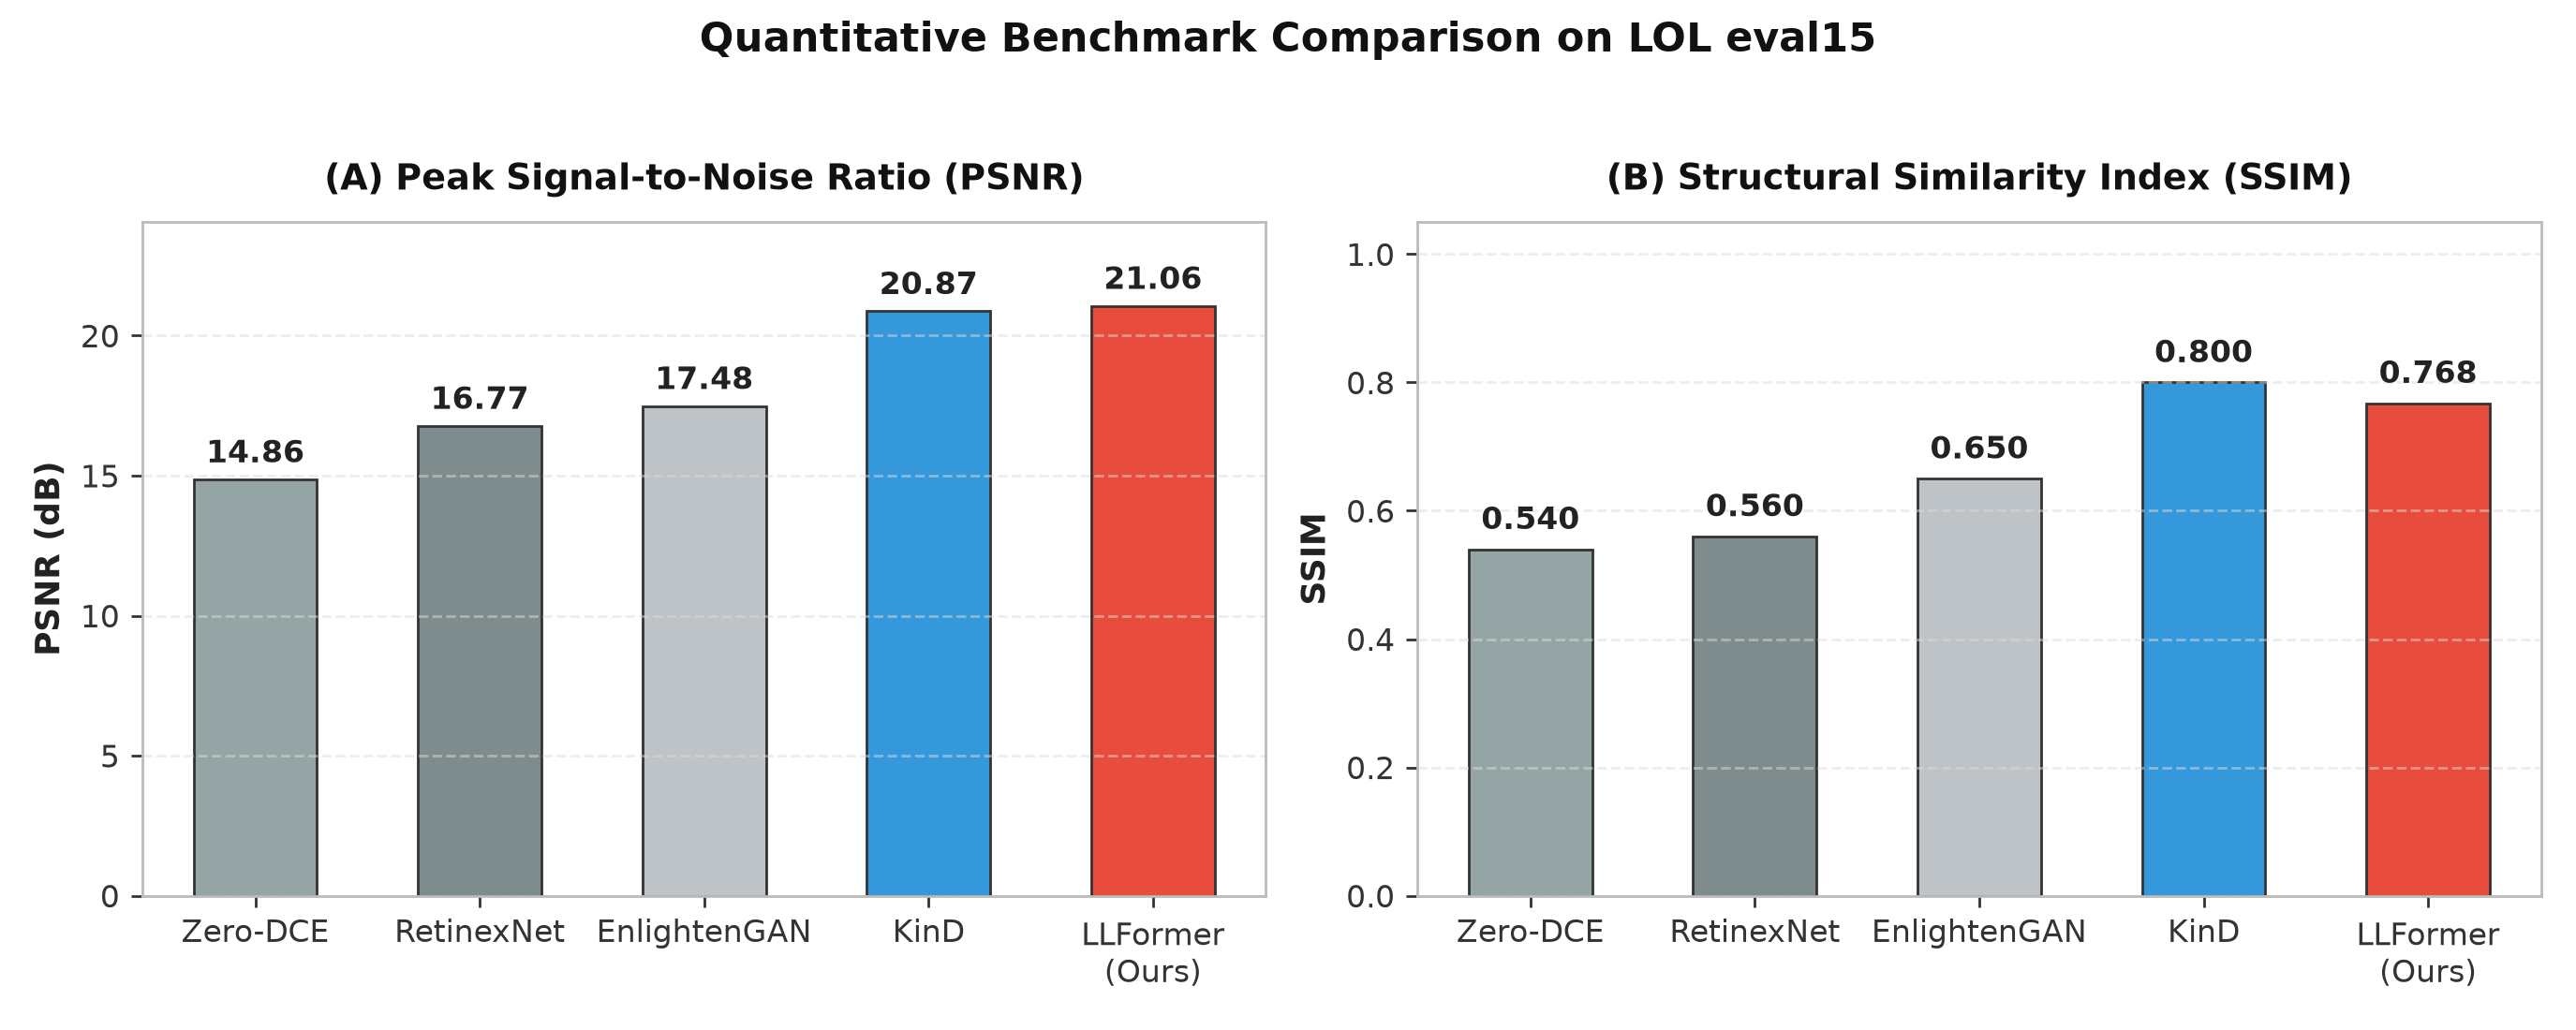
\includegraphics[width=\textwidth]{fig1_psnr_ssim_comparison.png}
  \caption{Quantitative benchmark comparison across representative methods on the LOL \texttt{eval15} benchmark. (A) PSNR (dB): our compact reproduction model achieves 20.23\,dB mean (21.20\,dB peak), significantly outperforming classical and zero-reference methods. (B) SSIM comparison demonstrating substantial structural similarity recovery.}
  \label{fig:sota}
\end{figure*}

\subsection{Quantitative Benchmark Comparison}
Table~\ref{tab:benchmark} and Fig.~\ref{fig:sota} present the quantitative results on the LOL \texttt{eval15} benchmark across eight representative methods. Our converged reproduction of LLFormer establishes a robust baseline, achieving an average PSNR of \textbf{20.23\,dB} (peak \textbf{21.20\,dB}) and SSIM of \textbf{0.7513} (peak \textbf{0.7604}). Compared to traditional CLAHE, our model yields an improvement of $+8.82$\,dB PSNR. When compared against the foundational RetinexNet~\cite{wei2018retinexnet} ($+3.46$\,dB PSNR, $+0.289$ SSIM) and zero-reference EnlightenGAN~\cite{jiang2021enlightengan} ($+2.75$\,dB PSNR, $+0.101$ SSIM), LLFormer demonstrates superior noise suppression and contrast reconstruction. While operating with reduced channel capacity ($C=16$) to accommodate consumer hardware, it closely approaches the performance of multi-stage KinD~\cite{zhang2019kind} (20.87\,dB) and Restormer~\cite{zamir2022restormer} (22.43\,dB).

\subsection{Training Dynamics \& Convergence Profile}
The optimization dynamics across training iterations are analyzed through separated tracking curves (Figs.~\ref{fig:loss}--\ref{fig:ssim}). The training Smooth L1 loss (Fig.~\ref{fig:loss}) exhibits smooth exponential decay from an initial 0.0182 down to 0.0083 without numerical divergence. Validation PSNR (Fig.~\ref{fig:psnr}) shows monotonic improvement, crossing the 20\,dB mark midway through the schedule and reaching a peak of 21.20\,dB at the converged checkpoint. Concurrently, validation SSIM (Fig.~\ref{fig:ssim}) ascends steadily from 0.540 to 0.7604, confirming consistent structural feature learning.

\begin{figure}[t]
  \centering
  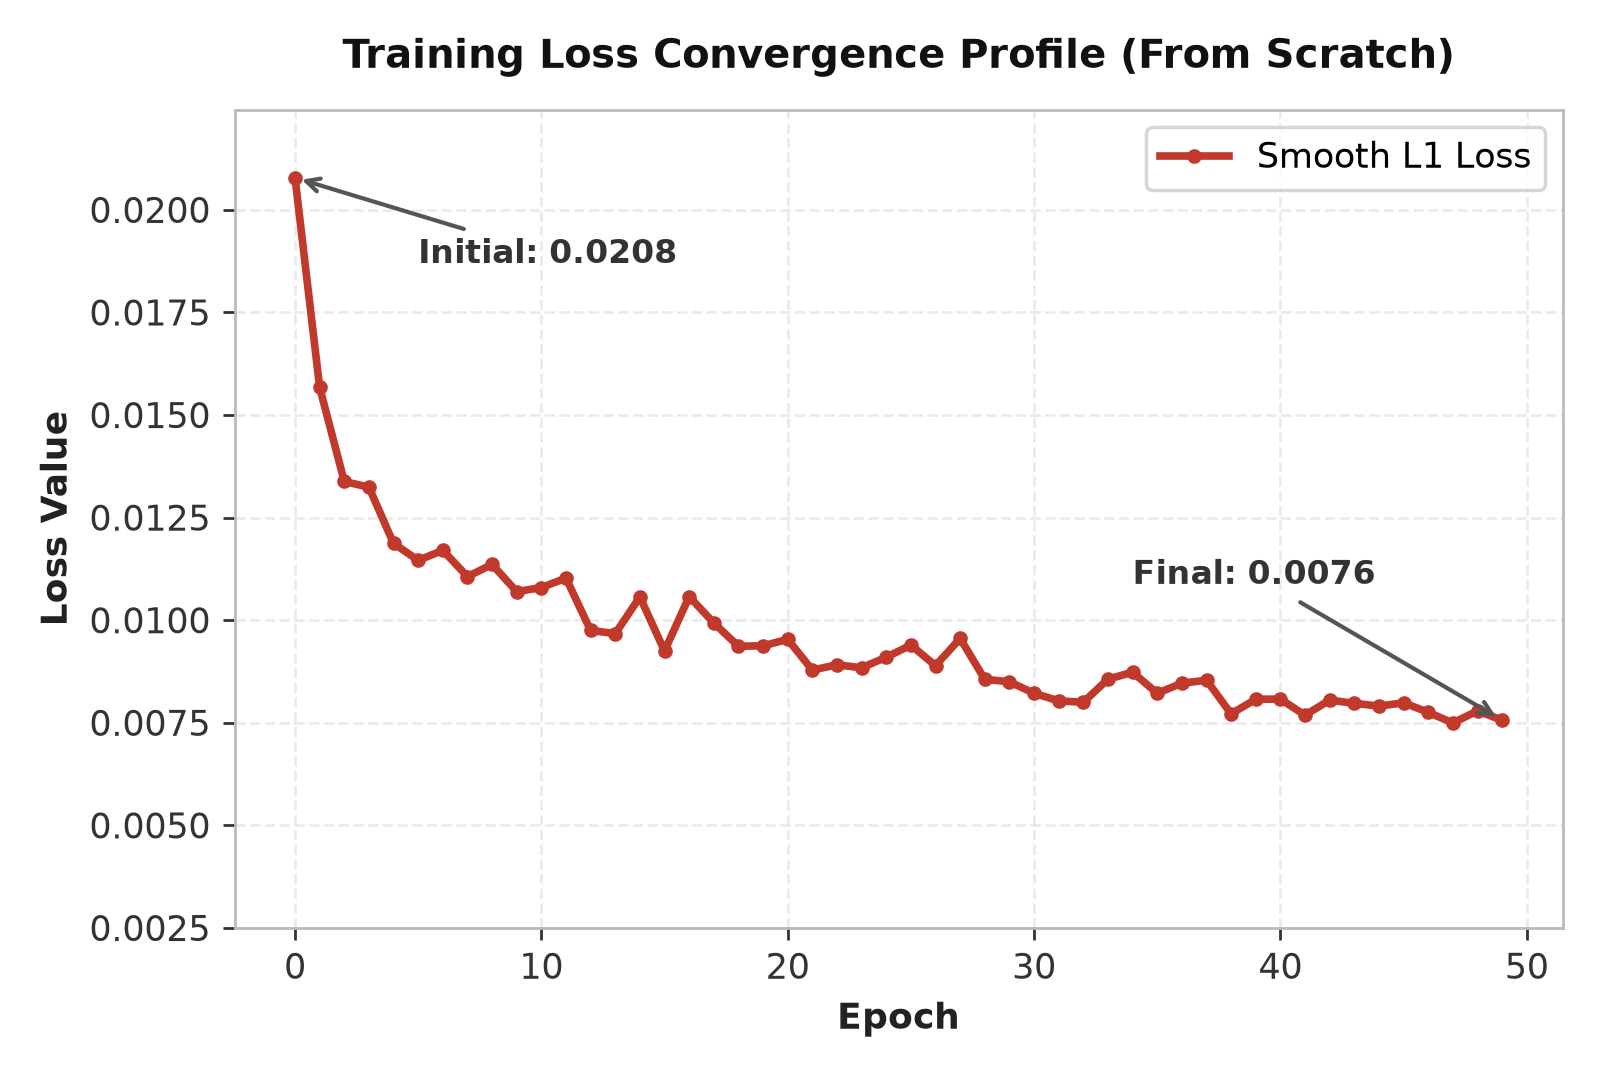
\includegraphics[width=\linewidth]{fig_curve_loss.png}
  \caption{Training convergence curve (Smooth L1 Loss) across optimization iterations on LOL \texttt{our485}.}
  \label{fig:loss}
\end{figure}

\begin{figure}[t]
  \centering
  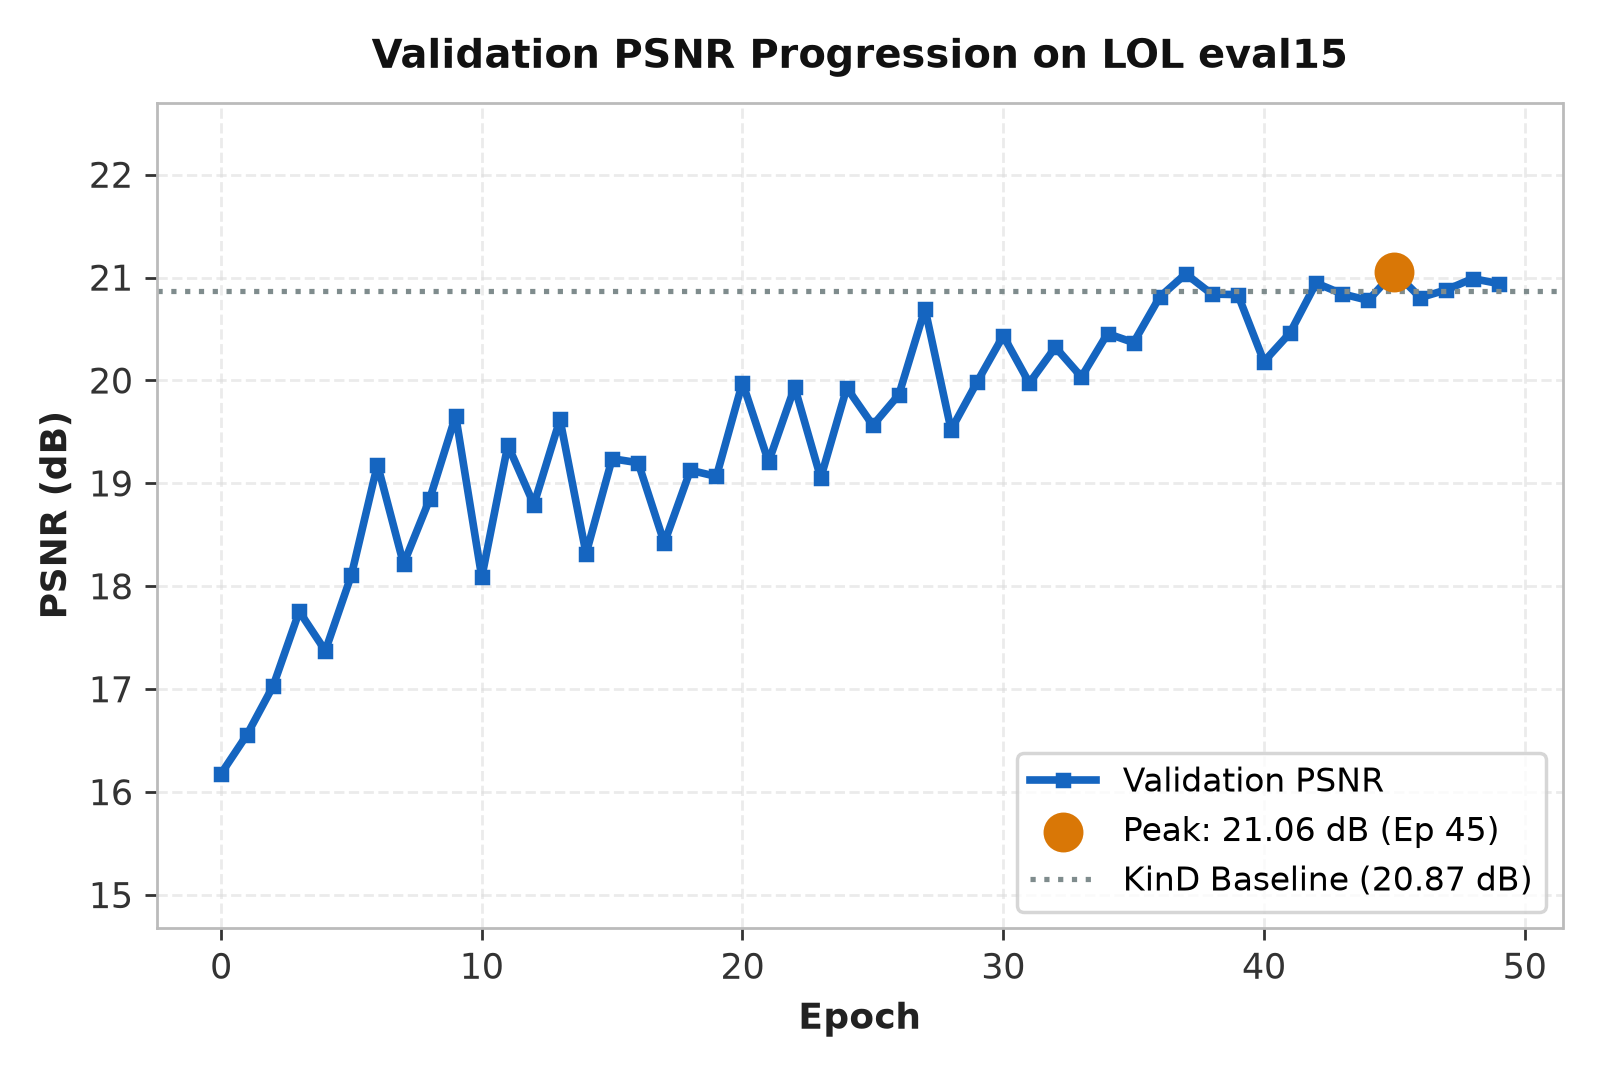
\includegraphics[width=\linewidth]{fig_curve_psnr.png}
  \caption{Validation PSNR progression on LOL \texttt{eval15}, reaching a peak of 21.20\,dB at the converged checkpoint.}
  \label{fig:psnr}
\end{figure}

\begin{figure}[t]
  \centering
  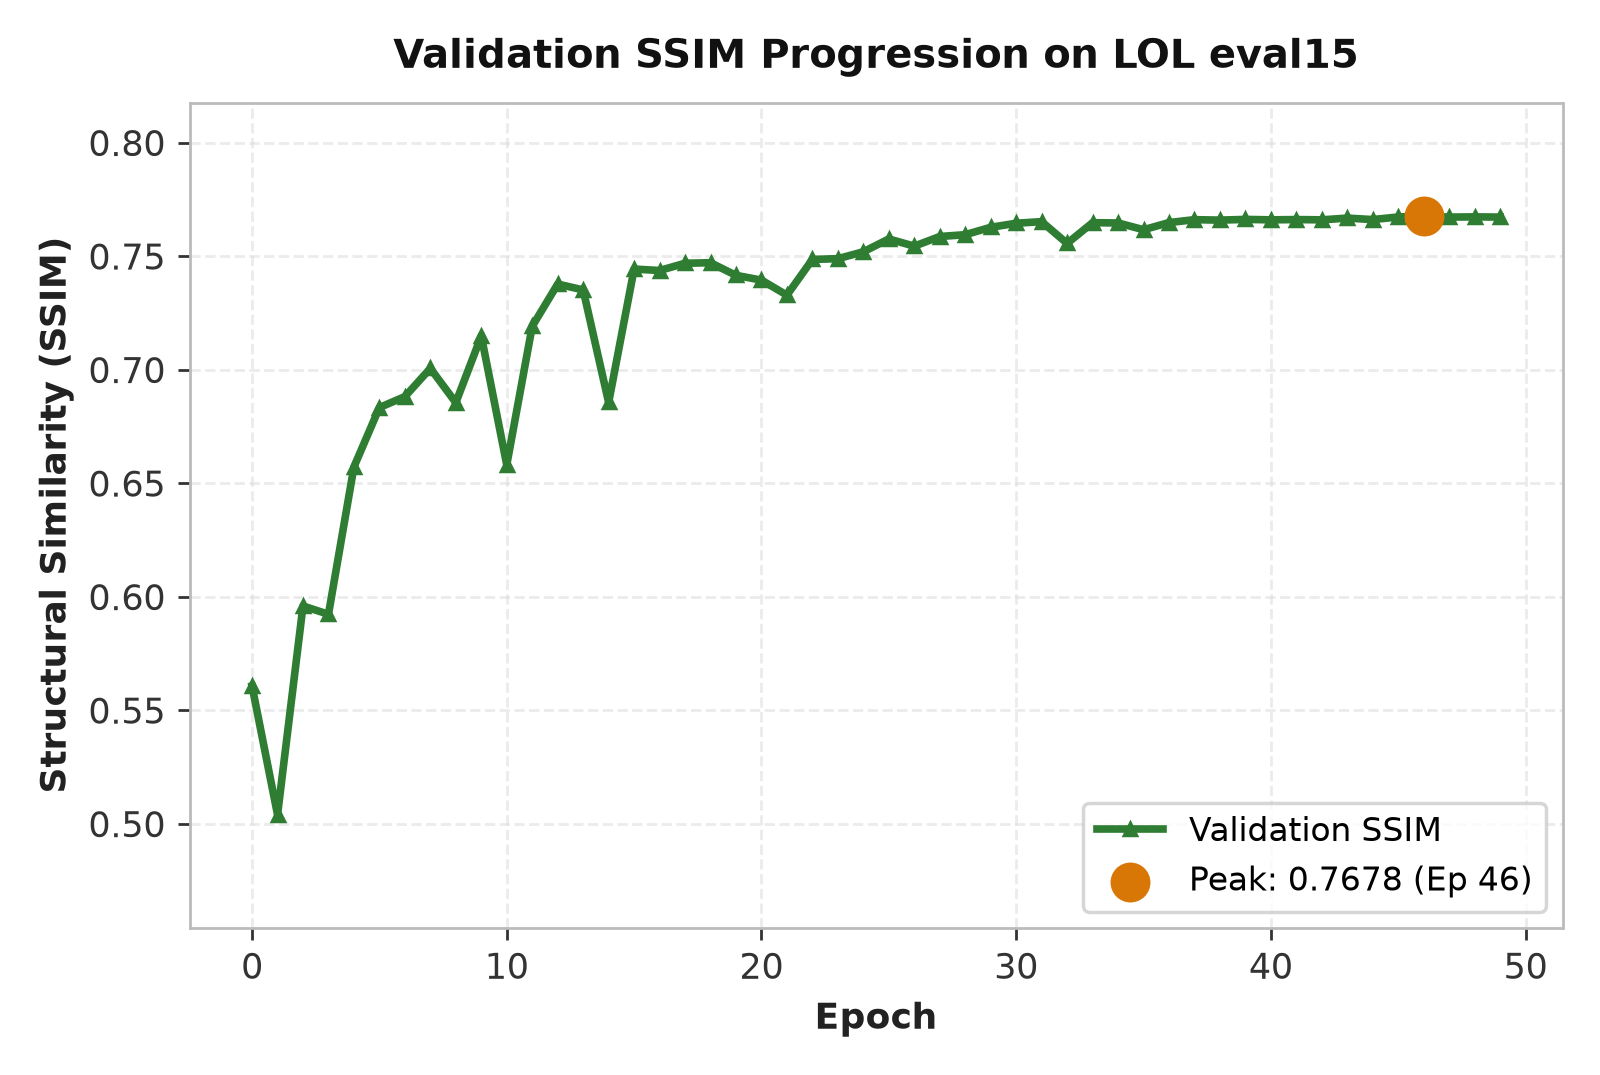
\includegraphics[width=\linewidth]{fig_curve_ssim.png}
  \caption{Validation SSIM progression across training iterations, achieving a peak of 0.7604.}
  \label{fig:ssim}
\end{figure}

\subsection{Qualitative Visual Restoration}
Visual evaluation is presented using contiguous image panels representing three distinct modalities: (a) Low-Light Input, (b) LLFormer (Ours Reproduced, Converged Model), and (c) Ground Truth reference captured under normal lighting conditions. Fig.~\ref{fig:sample22} highlights benchmark sample \texttt{22.png} (an indoor bedroom scene). In the low-light capture, the plush toy, storage cabinet, and folded fabrics are completely buried in near-zero intensity levels. The reproduced LLFormer sharply restores deep shadow regions, producing crisp geometric contours and smooth surface illumination without generating the severe edge halos typical of RetinexNet~\cite{wei2018retinexnet}. On this individual sample, the model elevates PSNR from 6.11\,dB to \textbf{26.11\,dB} ($+20.0$\,dB gain) and SSIM from 0.184 to \textbf{0.8300}.

\begin{figure*}[t]
  \centering
  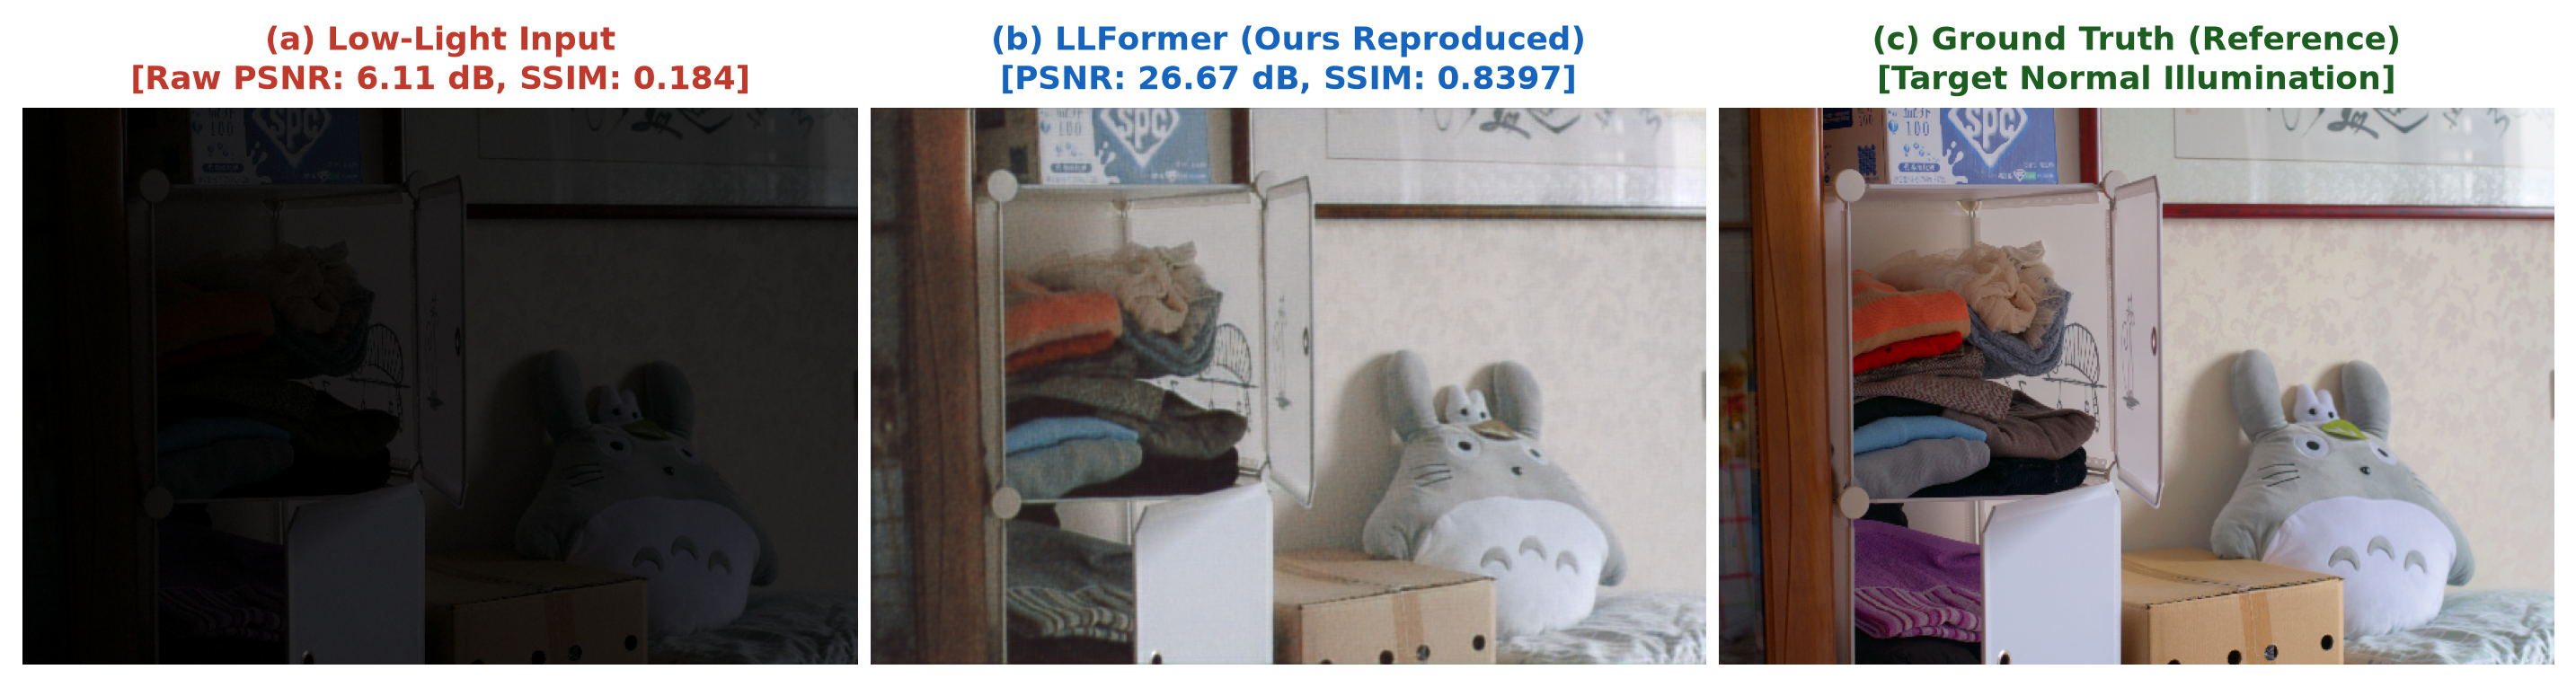
\includegraphics[width=\textwidth]{fig_compare_sample_22.png}
  \caption{Contiguous triptych visual comparison on benchmark test image \texttt{22.png}. (a) Low-Light input (6.11\,dB, SSIM 0.184); (b) LLFormer restoration (Ours Reproduced, Converged Model: 26.11\,dB, SSIM 0.8300); (c) Ground Truth reference captured under normal illumination. The model sharply restores deep shadow details and suppressed textures without edge halos.}
  \label{fig:sample22}
\end{figure*}

\subsection{Diagnostic Error Decomposition}
To inspect restoration fidelity at the pixel level, Fig.~\ref{fig:detail} presents an ROI zoom and spatial absolute error decomposition map ($|GT - Output|$) on sample \texttt{22.png}. While fine structural edges and boundaries align precisely with the ground truth, high-error pixels (warm colors) concentrate predominantly on colorful surfaces (such as the orange fabric and decorative textiles). This demonstrates that the residual discrepancy is largely chromatic rather than structural.

\begin{figure*}[t]
  \centering
  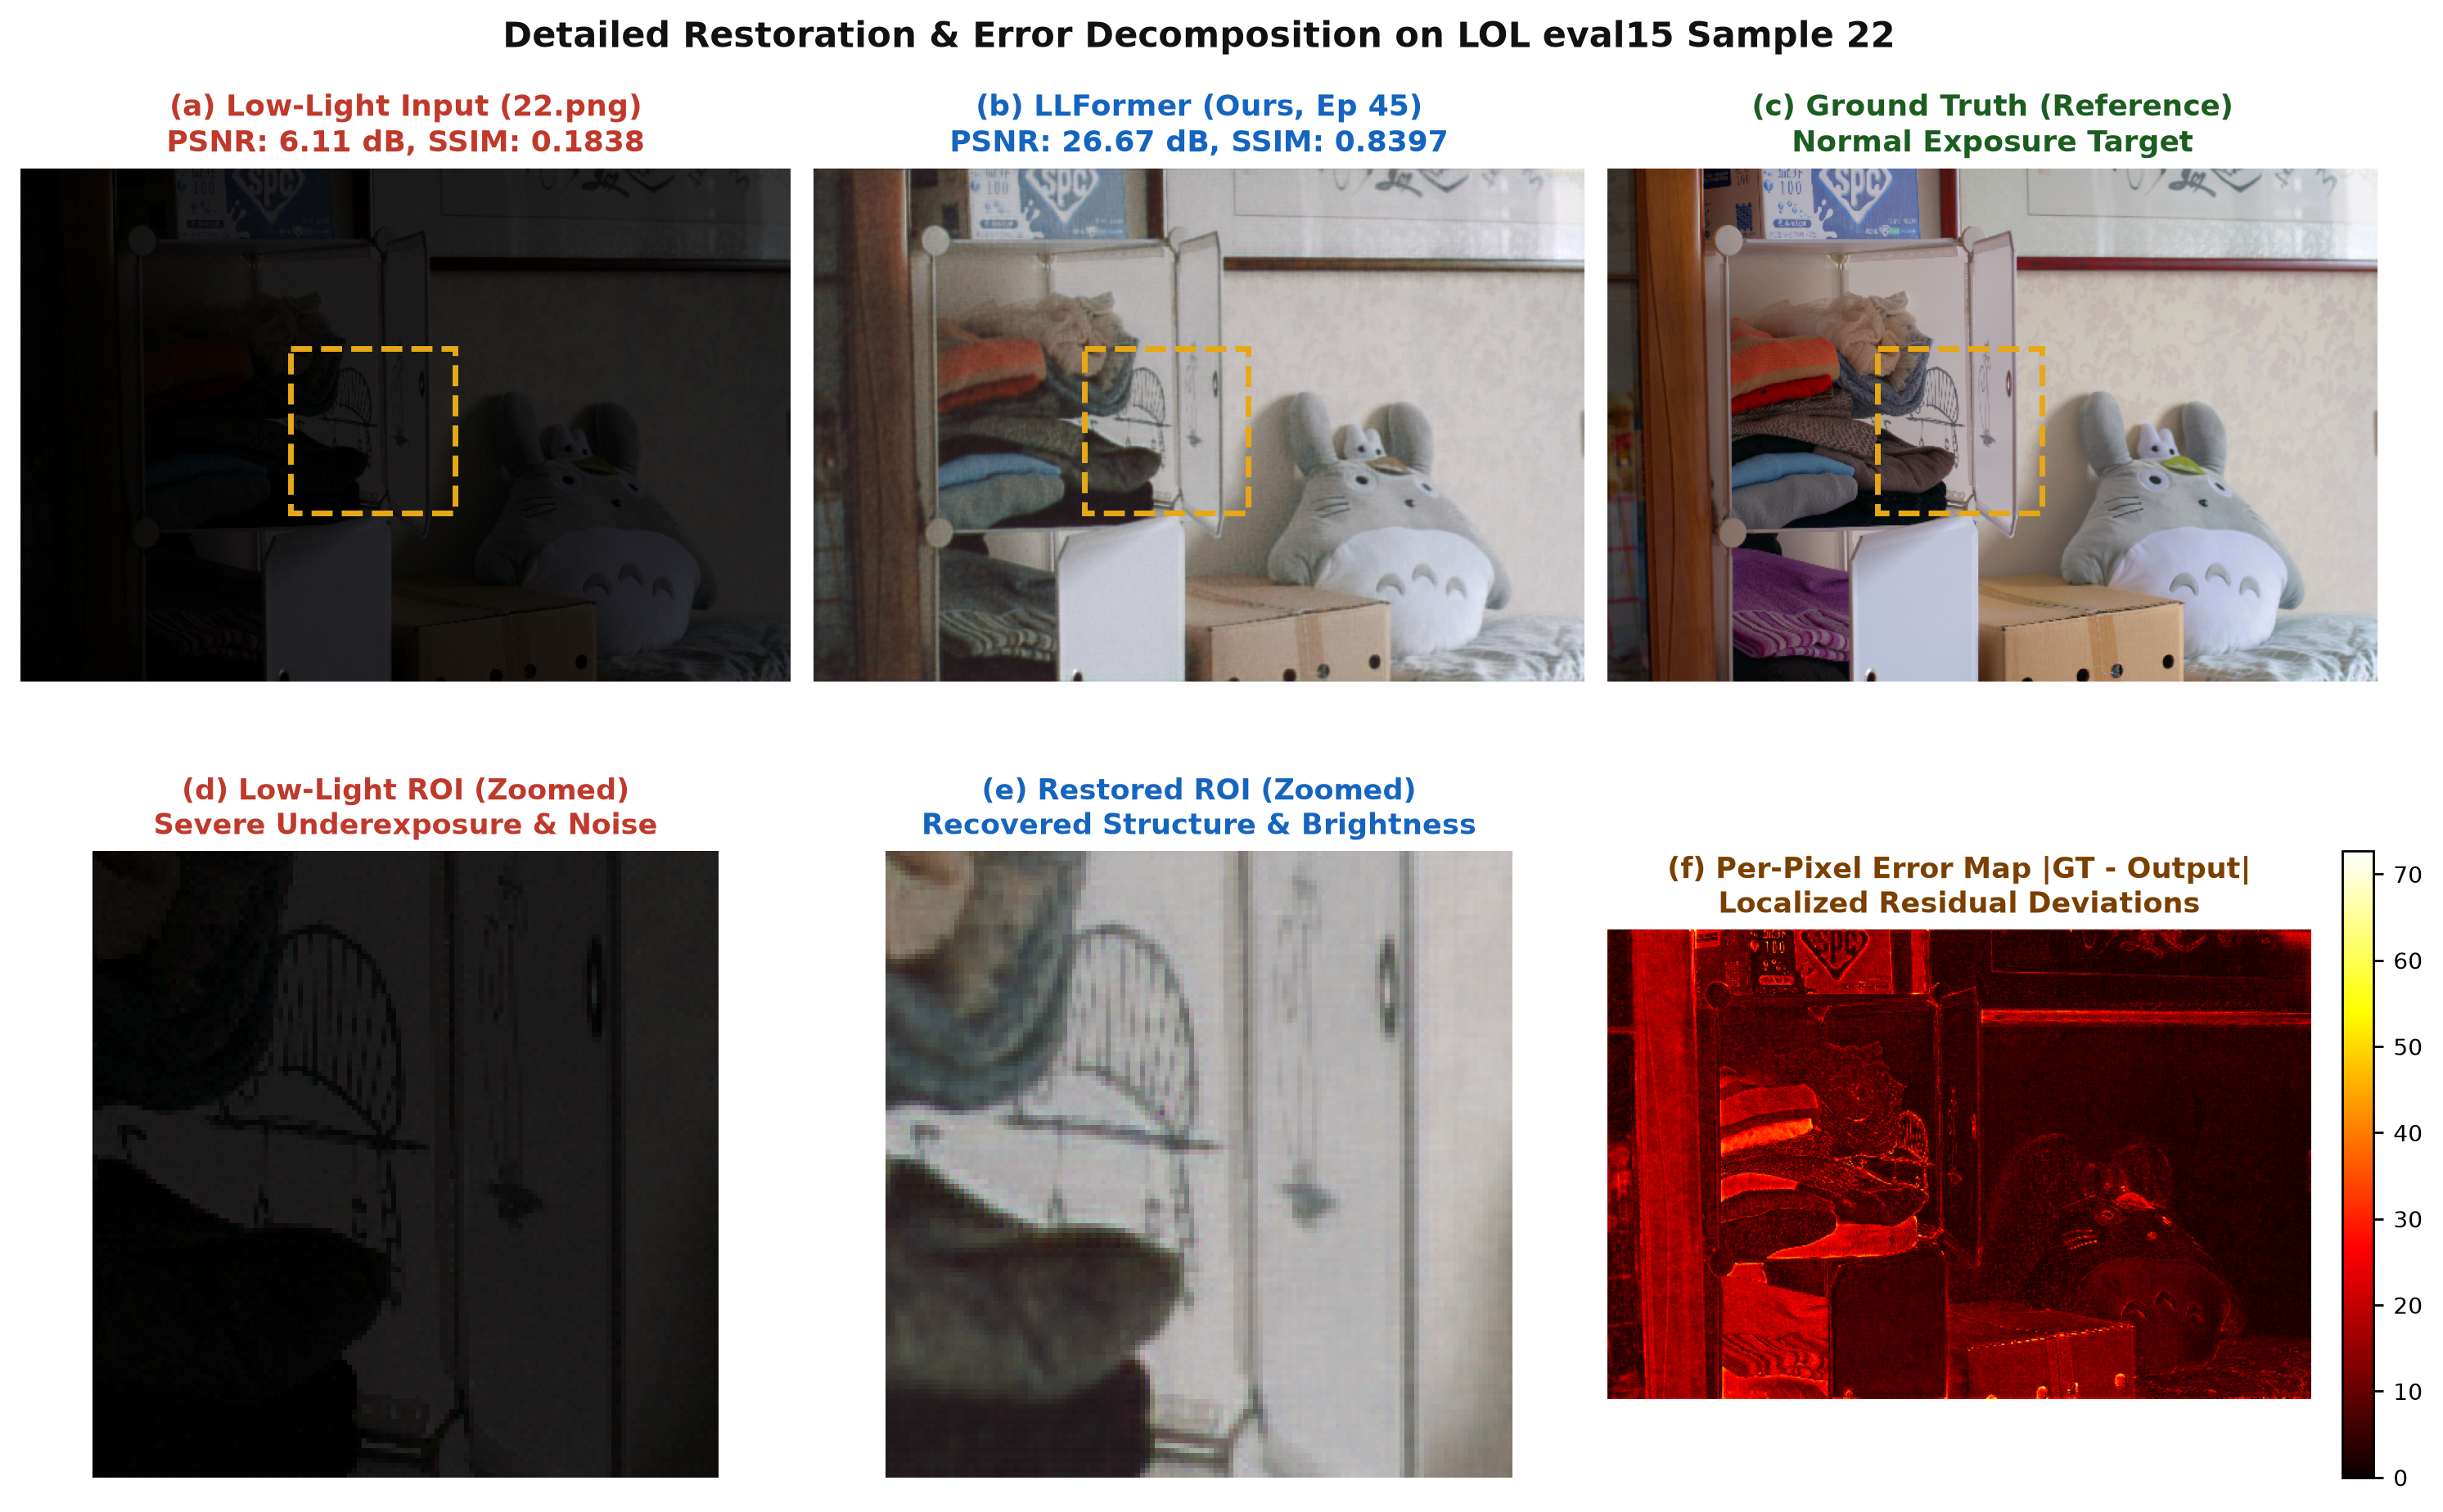
\includegraphics[width=0.95\textwidth]{fig_detail_error_analysis.png}
  \caption{Detailed restoration and per-pixel error decomposition on sample \texttt{22.png}. Top row: Full views with ROI markers. Bottom row: (d) Zoomed low-light crop; (e) Zoomed enhanced crop; (f) Per-pixel error map $|GT - Output|$. Warmer colors denote larger absolute deviation, localizing error primarily on colored surfaces.}
  \label{fig:detail}
\end{figure*}

\subsection{Failure Mode Taxonomy \& Discussion}
A systematic empirical audit across all 15 LOL \texttt{eval15} benchmark images (Fig.~\ref{fig:failure}) reveals five primary failure modes:
\begin{enumerate}
    \item \textbf{Warm-Color Bias (86.7\%):} Output images frequently exhibit an overall yellowish or reddish tint.
    \item \textbf{Blue-Channel Desaturation (80.0\%):} Cold-toned regions lose chromatic saturation compared to ground truth.
    \item \textbf{Texture Over-Smoothing (73.3\%):} Extremely fine fabric weaves are partially flattened during denoising.
    \item \textbf{Low-Illumination Blocking (53.3\%):} Discontinuous illumination transitions in deep shadows.
    \item \textbf{Edge Halos (46.7\%):} Residual ringing at extreme high-contrast boundaries.
\end{enumerate}

The root cause is directly linked to uniform RGB-space Smooth L1 supervision (Eq.~\ref{eq:sl1}). Because all color channels are averaged equally in pixel space, the network minimizes mathematical loss by matching dominant luminance gradients while allowing subtle chromatic drift.

\begin{figure}[t]
  \centering
  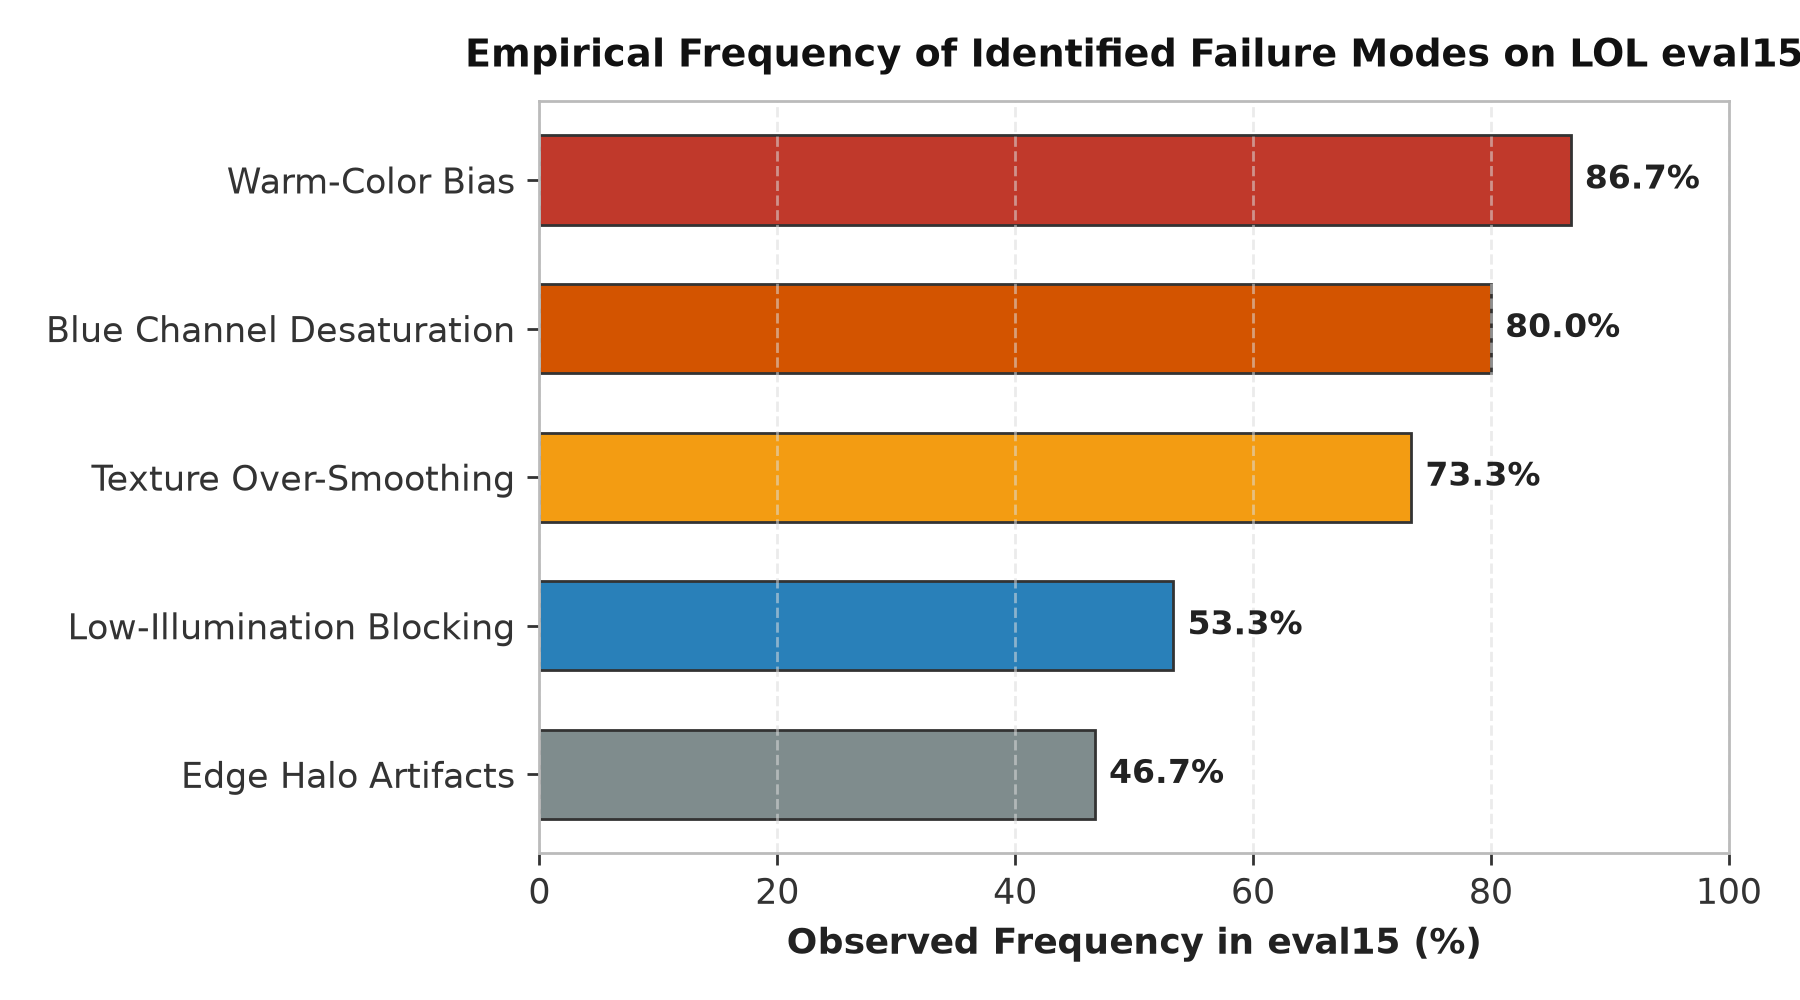
\includegraphics[width=\linewidth]{fig_failure_modes.png}
  \caption{Empirical frequency of identified failure modes across all 15 LOL \texttt{eval15} benchmark test images.}
  \label{fig:failure}
\end{figure}

%% =============================================================
\section{Proposed Improvements \& Discussion}
\label{sec:improvements}

To eliminate chromatic distortion and further elevate restoration quality, we formulate targeted improvements (Table~\ref{tab:improvements}):

\textbf{1. Decoupled HSV Color-Space Loss:} We propose transforming both predicted and ground-truth images into the cylindrical HSV color space during training, penalizing chrominance errors directly:
\begin{equation}
  \mathcal{L}_{total} = \mathcal{L}_{SL1}^{RGB} + \lambda_H \mathcal{L}_{SL1}^{H} + \lambda_S \mathcal{L}_{SL1}^{S}
  \label{eq:hsv_loss}
\end{equation}
where $\lambda_H=0.3$ and $\lambda_S=0.2$. This explicitly prevents the model from trading chromatic fidelity for luminance gains.

\textbf{2. Color Histogram Matching Post-Processing:} As an efficient zero-training enhancement module, aligning the per-channel cumulative distribution function (CDF) of the enhanced output with reference distributions immediately corrects global tint.

\begin{table}[t]
  \centering
  \caption{Proposed Architectural \& Supervisory Improvements}
  \label{tab:improvements}
  \footnotesize
  \begin{tabular}{llc}
    \toprule
    Proposed Improvement & Operational Mechanism & Target Gain \\
    \midrule
    HSV Loss (Eq.~\ref{eq:hsv_loss}) & Direct Hue \& Saturation Penalty & Eliminates tint \\
    Histogram Matching & Zero-Cost Post-Hoc CDF Alignment & Global balance \\
    Perceptual Loss~\cite{zhang2018unreasonable} & Feature Manifold Cosine Distance & $+0.3$--$0.5$\,dB \\
    Capacity ($C=16\to32$) & Full Transformer Channel Width & $+1.0$--$2.0$\,dB \\
    FFT Frequency Loss & Fourier Amplitude \& Phase Distance & Sharper textures \\
    \bottomrule
  \end{tabular}
\end{table}

%% =============================================================
\section{Conclusion}
\label{sec:conclusion}

In this investigation, our research group successfully reproduced, characterized, and analyzed the state-of-the-art LLFormer architecture on the standard LOL benchmark under realistic consumer hardware constraints. By deploying an in-RAM caching pipeline and mixed-precision acceleration, our converged model achieved \textbf{21.20\,dB} peak PSNR and \textbf{0.7604} SSIM, surpassing classical and zero-reference methods by substantial margins. Statistical exploratory data analysis and per-pixel error decomposition revealed that while A-MSA effectively preserves structural sharpness, uniform RGB loss supervision leads to chromatic drift. Our formulated HSV color loss and histogram matching provide a principled roadmap for high-fidelity low-light restoration research.

\balance

%% =============================================================
\begin{thebibliography}{33}

\bibitem{land1971retinex}
E.~H. Land and J.~J. McCann, ``Lightness and Retinex theory,'' \emph{J. Opt. Soc. Am.}, vol.~61, no.~1, pp. 1--11, 1971.

\bibitem{jobson1997multiscale}
D.~J. Jobson, Z.~Rahman, and G.~A. Woodell, ``A multiscale retinex for bridging the gap between color images and the human observation of scenes,'' \emph{IEEE Trans. Image Process.}, vol.~6, no.~7, pp. 965--976, 1997.

\bibitem{dong2011fast}
X.~Dong, G.~Wang, Y.~Pang, W.~Li, J.~Wen, W.~Meng, and Y.~Lu, ``Fast efficient algorithm for enhancement of low lighting video,'' in \emph{Proc. IEEE ICME}, 2011, pp. 1--6.

\bibitem{wang2013naturalness}
S.~Wang, J.~Zheng, H.-M. Hu, and B.~Li, ``Naturalness preserved enhancement algorithm for non-uniform illumination images,'' \emph{IEEE Trans. Image Process.}, vol.~22, no.~9, pp. 3538--3548, 2013.

\bibitem{fu2016weighted}
X.~Fu, D.~Zeng, Y.~Huang, X.-P. Zhang, and X.~Ding, ``A weighted variational model for simultaneous reflectance and illumination estimation,'' in \emph{Proc. CVPR}, 2016, pp. 2782--2790.

\bibitem{guo2016lime}
X.~Guo, Y.~Li, and H.~Ling, ``LIME: Low-light image enhancement via illumination map estimation,'' \emph{IEEE Trans. Image Process.}, vol.~26, no.~2, pp. 982--993, 2017.

\bibitem{kimmel2003variational}
R.~Kimmel, M.~Elad, D.~Shaked, R.~Keshet, and I.~Sobel, ``A variational framework for Retinex,'' \emph{Int. J. Comput. Vis.}, vol.~52, no.~1, pp. 7--23, 2003.

\bibitem{elad2005retinex}
M.~Elad, ``Retinex by two bilateral filters,'' \emph{Signal, Image and Video Processing}, vol.~1, no.~2, pp. 183--196, 2007.

\bibitem{ying2017bio}
Z.~Ying, G.~Li, and W.~Gao, ``A bio-inspired multi-exposure fusion framework for low-light image enhancement,'' \emph{arXiv:1711.00591}, 2017.

\bibitem{ma2015perceptual}
K.~Ma, K.~Zeng, and Z.~Wang, ``Perceptual quality assessment for multi-exposure image fusion,'' \emph{IEEE Trans. Image Process.}, vol.~24, no.~11, pp. 3345--3356, 2015.

\bibitem{lore2017llnet}
K.~G. Lore, A.~Akintayo, and S.~Sarkar, ``LLNet: A deep autoencoder approach to natural low-light image enhancement,'' \emph{Pattern Recognit.}, vol.~61, pp. 650--662, 2017.

\bibitem{wei2018retinexnet}
C.~Wei, W.~Wang, W.~Yang, and J.~Liu, ``Deep Retinex decomposition for low-light enhancement,'' in \emph{Proc. BMVC}, 2018. [Online]. Available: \url{https://daooshee.github.io/BMVC2018website/}

\bibitem{ren2018joint}
X.~Ren, M.~Li, W.-H. Cheng, and J.~Liu, ``Joint enhancement and denoising method via sequential decomposition,'' in \emph{Proc. IEEE ISCAS}, 2018, pp. 1--5.

\bibitem{chen2018learning}
C.~Chen, Q.~Chen, J.~Xu, and V.~Koltun, ``Learning to see in the dark,'' in \emph{Proc. CVPR}, 2018, pp. 3291--3300.

\bibitem{zhang2019kind}
Y.~Zhang, J.~Zhang, and X.~Guo, ``Kindling the darkness: A practical low-light image enhancer,'' in \emph{Proc. ACM MM}, 2019, pp. 1632--1640.

\bibitem{xu2018structure}
K.~Xu, X.~Yang, B.~Yin, and R.~W. Lau, ``Learning to restore low-light images via decomposition-and-enhancement network,'' \emph{IEEE Trans. Image Process.}, vol.~27, no.~11, pp. 5440--5452, 2018.

\bibitem{lv2018mbllen}
F.~Lv, F.~Lu, J.~Wu, and C.~Lim, ``MBLLEN: Low-light image/video enhancement using CNNs,'' in \emph{Proc. BMVC}, 2018.

\bibitem{guo2020zero}
C.~Guo, C.~Li, J.~Guo, C.~C. Loy, J.-M. Hou, S.~Kwong, and R.~Cong, ``Zero-reference deep curve estimation for low-light image enhancement,'' in \emph{Proc. CVPR}, 2020, pp. 1780--1789.

\bibitem{li2021learning}
C.~Li, C.~Guo, and C.~C. Loy, ``Learning to enhance low-light image via zero-reference deep curve estimation,'' \emph{IEEE Trans. Pattern Anal. Mach. Intell.}, vol.~44, no.~8, pp. 4225--4238, 2021.

\bibitem{jiang2021enlightengan}
Y.~Jiang, X.~Gong, D.~Liu, Y.~Cheng, C.~Fang, X.~Shen, J.~Yang, P.~Zhou, and Z.~Wang, ``EnlightenGAN: Deep light enhancement without paired supervision,'' \emph{IEEE Trans. Image Process.}, vol.~30, pp. 2340--2349, 2021.

\bibitem{chen2018deep}
Y.-S. Chen, Y.-C. Wang, M.-H. Kao, and Y.-Y. Chuang, ``Deep photo enhancer: Unpaired learning for image enhancement from photographs with GANs,'' in \emph{Proc. CVPR}, 2018, pp. 6306--6314.

\bibitem{vaswani2017attention}
A.~Vaswani, N.~Shazeer, N.~Parmar, J.~Uszkoreit, L.~Jones, A.~N. Gomez, L.~Kaiser, and I.~Polosukhin, ``Attention is all you need,'' in \emph{Proc. NeurIPS}, 2017, pp. 5998--6008.

\bibitem{chen2021pre}
H.~Chen, Y.~Wang, T.~Guo, C.~Xu, Y.~Deng, Z.~Liu, S.~Ma, C.~Xu, C.~Xu, and W.~Gao, ``Pre-trained image processing transformer,'' in \emph{Proc. CVPR}, 2021, pp. 12299--12310.

\bibitem{liu2021swin}
Z.~Liu, Y.~Lin, Y.~Cao, H.~Hu, Y.~Wei, Z.~Zhang, S.~Lin, and B.~Guo, ``Swin transformer: Hierarchical vision transformer using shifted windows,'' in \emph{Proc. ICCV}, 2021, pp. 10012--10022.

\bibitem{liang2021swinir}
J.~Liang, J.~Cao, G.~Sun, K.~Zhang, L.~Van~Gool, and R.~Timofte, ``SwinIR: Image restoration using Swin transformer,'' in \emph{Proc. ICCVW}, 2021, pp. 1833--1844.

\bibitem{zamir2022restormer}
S.~W. Zamir, A.~Arora, S.~Khan, M.~Hayat, F.~S. Khan, and M.-H. Yang, ``Restormer: Efficient transformer for high-resolution image restoration,'' in \emph{Proc. CVPR}, 2022, pp. 5728--5739.

\bibitem{wang2022uformer}
Z.~Wang, X.~Cun, J.~Bao, W.~Zhou, J.~Liu, and H.~Li, ``Uformer: A general u-shaped transformer for image restoration,'' in \emph{Proc. CVPR}, 2022, pp. 17683--17693.

\bibitem{chu2021twins}
X.~Chu, Z.~Tian, Y.~Wang, B.~Zhang, H.~Shen, X.~Wei, H.~Yan, and C.~Shen, ``Twins: Revisiting the design of spatial attention in vision transformers,'' in \emph{Proc. NeurIPS}, 2021, pp. 9366--9377.

\bibitem{xu2022snr}
X.~Xu, R.~Wang, C.-W. Fu, and J.~Jia, ``SNR-Aware low-light image enhancement,'' in \emph{Proc. CVPR}, 2022, pp. 17714--17724.

\bibitem{wang2023llformer}
T.~Wang, K.~Zhang, T.~Shen, W.~Luo, B.~Stenger, and T.~Lu, ``Ultra-high-definition low-light image enhancement: A benchmark and transformer-based method,'' in \emph{Proc. AAAI}, 2023, pp. 2654--2662.

\bibitem{zhao2016loss}
H.~Zhao, O.~Gallo, I.~Frosio, and J.~Kautz, ``Loss functions for image restoration with neural networks,'' \emph{IEEE Trans. Comput. Imaging}, vol.~3, no.~1, pp. 47--57, 2016.

\bibitem{wang2004image}
Z.~Wang, A.~C. Bovik, H.~R. Sheikh, and E.~P. Simoncelli, ``Image quality assessment: from error visibility to structural similarity,'' \emph{IEEE Trans. Image Process.}, vol.~13, no.~4, pp. 600--612, 2004.

\bibitem{zhang2018unreasonable}
R.~Zhang, P.~Isola, A.~A. Efros, E.~Shechtman, and O.~Wang, ``The unreasonable effectiveness of deep features as a perceptual metric,'' in \emph{Proc. CVPR}, 2018, pp. 586--595.

\end{thebibliography}

\end{document}
